\chapter{Implementation}
\label{Implementation}

% % For off the shelf technologies, add in how they work

% Add in key challenges, tell story

    \section{Software Engineering Process}
    
        \subsection{Github}
        Github \citep{website:Github} was used to store and manage version control of the project. Moreover, Github's issue system was used to manage to do tasks throughout the project. The project's repository can be found here:
        \begin{itemize}
            \item \url{https://github.com/2312420/lvl4-project} 
        \end{itemize}
          
            \subsubsection{Issue Strategy}
            Issues were created based on a single overarching goal that had to be completed. Within the Issue, various tasks and steps were added that needed to be completed to achieve this goal. Issues would be created at the start of each week with the goal being to complete issues by the end of the week. This helped to keep a manageable number of issues at any given time and also allowed for easy oversight of how many issues remained from previous weeks. 
            
            \subsubsection{Commit and Branching Strategy}
            Commits were to be made every time one of the tasks in an issue was completed or an important step towards completing a task was taken. Commit messages were also kept small and concise in order to reduce confusion. A master and develop branch were initially created when work began on the project and these two branches existed throughout the projects life-cycle. When work began on an Issue, a new feature branch was created from develop. When the feature and goals for that issue had been achieved, the branch was merged into develop.
            
            All branches were named to abide by the following naming convention: "<name of issue / area being worked on>-<issue id>". For example Issue, \#58 "Prediction Restructure" branch would be named "Prediction\_Restructure-58". Merge requests were only ever made through the GitHub website so if any merge conflicts were raised, they could be easily solved. Each merge request was also referenced to the issue or issues it solved. Having a core branch and commit strategy helped to prevent the project repository from becoming too complex with an overabundance of branches while also still keeping the main and develop branches safely.
            
            \subsubsection{Repository Insights}
            Throughout the project's life cycle, 37 issues were created, 42 branches and branch merges were issued and 274 commits were made. Figure\ref{fig:Git_commmits} shows the commits made throughout the project. As we can see commits and work on the project were made consistently across the year:
            
            \begin{figure}
                \centering
                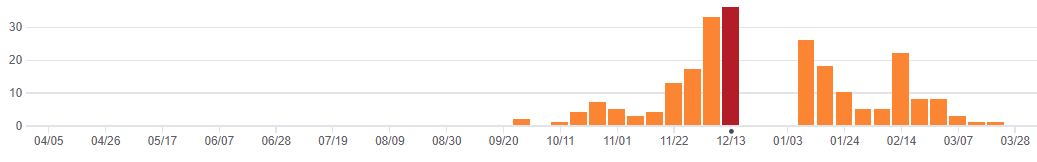
\includegraphics[width=\linewidth]{images/Commits.png}
                \caption{Overview of commits made to the project repository}
                \label{fig:Git_commmits}
            \end{figure}
            
        \subsection{Confluence}
        To organise weekly meetings and project notes, confluence \citep{website:confluence} was used, as it provides a whole host of note-taking features and allows for notes to be referenced and linked to one another to create a wiki for the project. A central page was set up for the project that contained connections to the various weekly notes. A project road map \ref{fig:Confluence_Roadmap} was also set up that contained a rough outline of what was done in each week and what was projected to be done in the weeks to come. 
        
        \begin{figure}[!h]
            \centering
            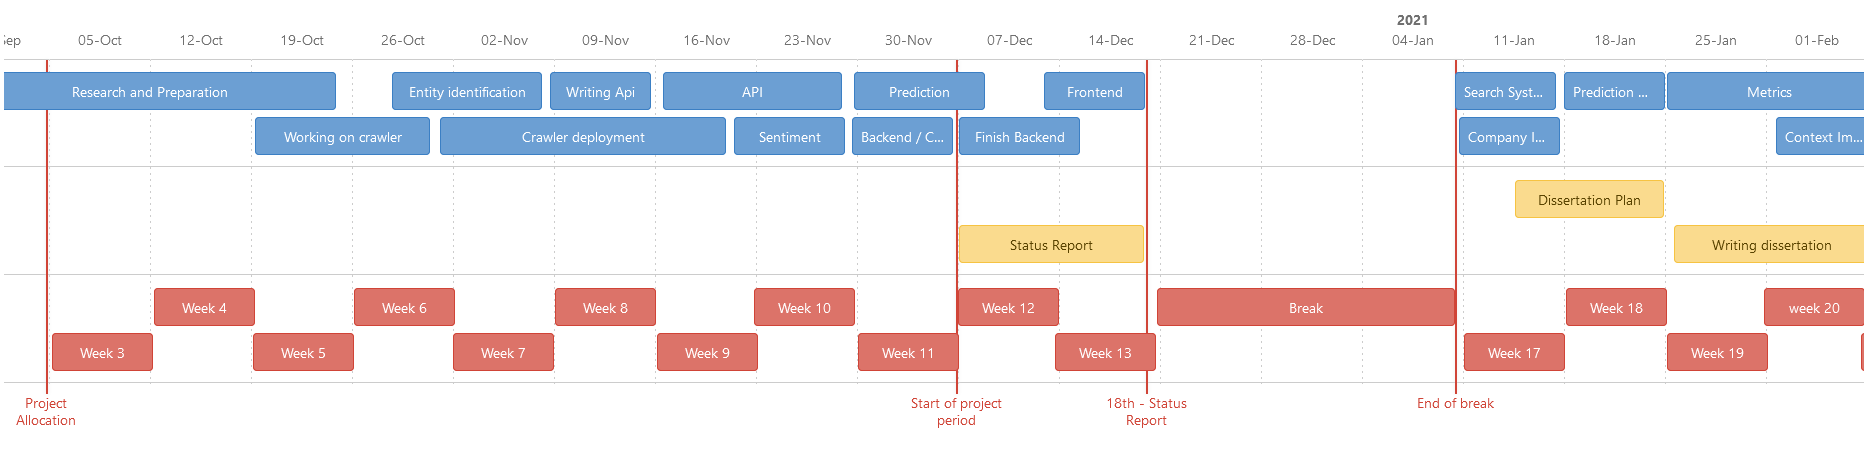
\includegraphics[width=0.9\linewidth]{images/upload/Roadmap.png}    
            \caption{Confluence Roadmap}
            \label{fig:Confluence_Roadmap}
        \end{figure}
        
        Additionally, on this home page was a list of all the project's requirements along with their importance (Must, Should, Could") and status (Done or Todo). This served as a constant reminder of the various key aspects of the project that still needed done and helped to stop the project from getting off-track or too focused on one requirement. 
        
        
    \section{Backend Implementation}
    Before the web app and its features could be created, the backend system first had to be up and running and therefore that is where the focus lay for the first months of the project. The backend components were built using Flask \citep{technology:Flask}, which allows the components to open up defined API calls.
    
        \subsection{News Crawler}
        % REDONE, sort of
        The news crawler is responsible for collecting articles from various sources, which will be processed and used throughout the system. Having data to test and work with while developing the other components was critical. It was therefore decided that the news crawler should be created first, since it is the logical starting point for articles in the system and provides access to this data. The crawler was implemented using the python library Newspaper3k \citep{technology:Newspaper} which provides simple methods and functions to scrape articles from News-sites RSS feeds. The news crawler will request articles from the various News sites until no new articles are found, when this happens the crawler sleeps for five minutes so as to not overload requests to the various sources. The Newscrawler communicates directly with the database through the backend API, inputting any new articles it manages to crawl
        
        \subsubsection{Redundancy} To prevent the same Articles from being inserted into the system, Articles are first put into a hash function that takes the first word of the article, the title of the article and the last word of the article to produce a unique ID. The article can then only be inserted into the system if this ID does not already exist.
        
        \begin{itemize}
            \item \textbf{Output}: \{title: "Stocks Today", transcript: "Apple's stocks fall today. Microsoft's stocks rise today", source\_id: "4"\}
        \end{itemize}    
            
        \subsection{Sentence Extraction}
        %REDONE
        The sentence extraction component is used to take the transcript of an article, extract the sentences from that article and return the list of sentences. The first step in creating the component was to implement the sentence extraction model which carries out the main function of separating the article into individual sentences. As mentioned in section \ref{des:sentence}, the extraction model was to be implemented using a pre-built model. Multiple technologies were considered, however NLTK \cite{Technology:NLTK} was decided upon as it offered extensive documentation, along with fast and simple implementation. NLTK provides multiple pre-trained models, each trained using a different data set. NLTK's Punkt sentence tokenizer was used to divide text into a list of sentences. This works by using an unsupervised learning algorithm which is trained in using large volumes of text. This algorithm develops a model which uses keywords, punctuation and phrases to divide text into sentences. With the sentence extraction method complete, the next step was to create the flask framework which exposes the necessary API calls for the system. The sentence extraction component contains one API exposed on its port, so that when given an article object in the form of a JSON, it returns a JSON of the sentences in the article.
        
        \begin{itemize}
            \item \textbf{Input}: \{transcript: "Apple's stocks fall today. Microsoft's stocks rise today"\}
            \item \textbf{Output}: \{["Apples stocks fall today", "Microsoft's stocks rise today"]\}
        \end{itemize}
        
        
        \subsection{Context Analysis}
        %REDONE
        The context analysis component is used to understand what company is being discussed in each article or sentence. The context analysis component when given an article needs to return a list of potential companies and when given a sentence needs to return the stock code of the company being discussed. As mentioned in section \ref{des:context} the context analysis component uses named entity recognition to identify the companies being discussed. This model was implemented using Spacy \cite{technology:Spacy} through its inbuilt word tokenization and NER model. Spacy was used initially as it had extensive documentation and could be implemented easily, however other technologies would be considered when the time came to evaluate the component. Spacy's named entity recognition model is trained using blogs and news articles and, as detailed in its documentation \cite{spacy_ner}, uses a neural network based approach to give analysis of sentences and label potential entities. With the named entity recognition model implemented, the context analysis component then separates out entities which do not have the "ORGANISATION" tag, as we are only interested in articles discussing companies. With the component able to identify companies being discussed in a text, the next step was to implement the flask framework and expose the two API calls for article and sentence context analysis. Articles and sentences are handled separately by the component:
        
            \subsubsection{Article Context}
            The article API call will use the NER model to analyze the transcript of the article and find any organisation entities it contains. When sent a JSON of the article, it will return the JSON with an additional "context" field which contains a list of potential entities being discussed in the article.
            
            \begin{itemize}
                \item \textbf{Input}: \{transcript: "Apple's stocks fall today. Microsoft's stocks rise today."\} 
                \item \textbf{Output}: \{transcript: "Apple's stocks fall today. Microsoft's stocks rise today." context: [Apple, Microsoft]\} 
            \end{itemize}
            
         
            \subsubsection{Sentence Context}
            The sentence API call also uses the NER model to analyze the text of the sentence to find any organisation entities it contains. If one or more organisations are found then that will be used as the potential context of the sentence. If no organisation is found then the sentences parent article context list is used instead. This is done to capture sentences that do not necessarily mention a company, but relate to the overall article context. Once the potential context of the sentence has been decided, it then needs to be linked to an item in the database. This was achieved by fuzzy querying the company database to find company short-hands that are similar to the potential entities. If the query manages to produce a valid result, then the stock code of that company becomes the context for the sentence. The text and new context of the sentence is then returned.
            
            \begin{itemize}
                \item \textbf{Input}: \{text:"Microsoft's stocks rise today"\}
                \item \textbf{Output}: \{text:"Microsoft's stocks rise today", context: "MSFT"\}
            \end{itemize}
            
            \subsubsection{Improvements}
            The context analysis component was improved by evaluating the effectiveness of the named entity recognition model, comparing the Spacy model to other technologies. The Stanford NER Libary, stanza \citep{technology:Stanza}, at the time of development contained more advanced fully neural network model that provided the best results, so the component was updated to use that model instead. More detail for the evaluation of the component can be found in chapter \ref{eval:context}
            
            
        \subsection{Sentiment Analysis}
        %REDONE
        The sentiment analysis component is used to analyze the text of a sentence and award a polarity score ranging from -1 to 1 on the sentiment of that text. It is one of the more important components as the score awarded here will be used in the stock prediction component. The sentiment analysis model was initially built using the python library VADER sentiment \citep{Technology:Vader}. This library provides open-source sentiment analysis tools to measure the sentiment intensity of a given text. This is done through a lexicon that scores positive and negative sentiment intensities for thousands of different words. This lexicon is then used to measure the amount of positive and negative words in a sentence and award a sentiment score. Once the VADER sentiment model was implemented, the next step was to again implement the framework and expose the API call that, when given text, returns the sentiment score. 
        
            \begin{itemize}
                \item \textbf{Input}: \{text:"Microsoft's stocks rise today"\}
                \item \textbf{Output}: \{score: "0.8"\}
            \end{itemize}
        
            \subsubsection{Improvements}
            Though VADER sentiment proved useful to build the initial sentiment analysis component we needed to ensure that the sentiment scores had a high degree of accuracy. Therefore VADER sentiment was compared to technologies in the paper Choosing your weapons: On sentiment analysis tools for software engineering research" \citep{7332508} mentioned in chapter \ref{Background}. The accuracy, precision and recall of each technology were measured, with Textblob \cite{technology:Textblob} providing the best results, the sentiment analysis component was then switch to use is sentiment model instead. Further details on the evaluation of the component can be found in chapter \ref{eval:sentiment}
        
       
       
        \subsection{Stock Prediction}
        The stock prediction component was one of the more complex and difficult parts of the system to implement and required significantly more time and work than the previous components. Sklearn \citep{technology:Scikit-learn} was used extensively throughout the component to provide the various predictions models needed.
            
            \subsubsection{Financial Data} The first step in creating the prediction model was to make it able to retrieve historical financial information about a given company. The python library Yfianance \citep{technology:yfinance} was used to retrieve financial information from Yahoo \citep{website:Yahoo}. Once the financial information is retrieved the component then gets the sentiment data collected on the company and combines the financial information and sentiment data into one. This proved difficult, as past a certain point financial data retrieved from Yahoo can only be collected by day rather than specific times. This required the sentient data to be averaged for each day before the combining process could begin. Once both data sets are ready a new data frame index by time is created, with the available financial and sentiment data filled in. 
            
            \subsubsection{Sentiment Prediction} The sentiment model is used to fill out the missing sentiment data in the previous data frame and to predict the future sentiment of the company. A sentiment model build using Sklearn's Bayesian Ridge regressor \cite{sklearn_bayes} uses known sentiment and financial data of the company to predict the missing sentiment data in the data frame. Once this is complete, the model then uses the dataframe to predict the future sentiment of the company by using the previous sentiment and the time separated into multiple features as training data. 
            
            \subsubsection{Stock Prediction} Once the dataframe with closing price, sentiment and time has been built, the component then moves onto predicting the potential future closing prices. Various models were evaluated to the best prediction results, with the final model being the Sklrean Random Forest Regressor \cite{sklearn_forest}, more information on this evaluation can be found in chapter \ref{eval:prediction}. A Random Forest Regressor is similar to a standard decision tree, in that it creates a tree of rules to decide the value of future data, however it has more randomness and variance to it, in order to avoid over fitting. 
            
            \subsubsection{Verdict}\label{Verdict} With the predictions having been made, the final step for the component is to analyze the data and award an overall verdict for the company. This is done by calculating the difference between the average of the predicted stock prices and the current stock price. If the difference is not greater than 0.5 or less than -0.5 then the stock is awarded the Hold verdict. A stock with a positive difference is awarded the Hot verdict whereas a stock with a negative difference is awarded the Not verdict. The difference, verdict and predictions are then returned. 
            
            \subsubsection{Custom Prediction and Restructure}
            The stock prediction component also had to facilitate user-made custom predictions. It was decided that a user would be able to define a start date and an end date and using any data in that time frame, the component would attempt to predict the stock prices. When the time came to implement this system, it became apparent that the stock prediction component had become confusing and disorganised with monolithic functions. It was therefore restructured with prediction models, data manipulation functions and common functions all being separated into their own files and directories. Additionally, various methods were expanded to accept a custom dates in order to better facilitate the custom prediction system. With this complete it a simple custom prediction function could be created with ease.

            \subsection{Overview} With the prediction system operational the stock prediction component was made to expose three API's using the Flask framework. The first API was the basic stock prediction used to determine the verdicts and information displayed on the web app:
            
            \begin{itemize}
                \item \textbf{Input}: \{stock\_code: "MSFT"\}
                \item \textbf{Output}: \{verdict: "HOT", predictions: [(01/04/2020, 102), ...]\}
            \end{itemize}
            
            The second is the custom prediction call that returns an ordered list of stock predictions between the start and end dates provided.
            
            \begin{itemize}
                \item \textbf{Input}: \{stock\_code: "MSFT", start\_date: "01\/04\/2020", end\_date:"01\/04\/2020"\}
                \item \textbf{Output} \{ predictions: [(01\/04\/2020, 102), ...] \}
            \end{itemize}
            
            Later in development the stock prediction component was expanded to contain an API call that transformed sentences into data points for the time series database. This was a straightforward implementation, with the input and output being:
            
            \begin{itemize}
                \item \textbf{Input} \{text:"Microsoft's stocks rise today", context: "MSFT", ..\}
                \item \textbf{Output} \{sentiment: "0.5", time: "01\/04\/2020", stock\_code: "MSFT, close\_price: 102"\}
            \end{itemize}
        
            
    \section{Database}
    The databases store the information that the system collects and process, with data split between the main database and the time-series database. The final schema for both databases can be found in Appendix \ref{fig:AP:schema}  
    
        \subsection{Main Database}
        The main database is used to store data on articles, sentences, companies and sources. PostgreSQL \citep{technology:PostgreSQL} was used to set up and manage the database as it is a well-known and long-established database management system with many features and good documentation to help guide the process of creating the database system. 
        
            \subsubsection{Tables}
            pgAdmin, a graphical extension that comes pre-packaged with PostgreSQL, was used to create the main database and the various tables it required. The Article, Sentence, Company and Source tables were created first with foreign key constraints linking them together. Each Article contained its source's ID, each sentence contained its parent article ID and each sentence also contained the stock code of the company it discussed, linking them together. When it came time to implement the Tag table, an intermediary table called Tags was created containing the ID of the tag and the stock code of the company it tagged. This created the desired many to many relationships between the Tag and Company table.
            
            \subsubsection{Inital Data}
            For the system to work, the company table had to be filled out with the shorthand names and stock codes of all the various companies. A data-set sourced from Kaggle, which contained the name and stock code of the S\&P 500 \citep{SP} was sourced to fill out this table. This data-set and more specifically, the S\&P 500 were selected due to them being some of the largest and most well-known companies in the world such as Apple, Amazon and Microsoft. The data set can be found here:
            \begin{itemize}
                \item \url{https://www.kaggle.com/dgawlik/nyse?select=securities.csv}
            \end{itemize}
            
        \subsection{Time-series Database}
        The Time-series database stores the data points used in the stock prediction component’s stock price prediction. Like the main database, the time-series database was implemented through PostgreSQL \citep{technology:PostgreSQL} however it only contains a single table which is the Datapoint table. To achieve the time-series functionality the Postgres extension Timescale \cite{technology:Timescale} was used is it allows for significantly faster and more accessible time-based queries to be made. 
        
            \subsubsection{Challenges}
            Timescale required a different version of PostgreSQL than the main database, meaning the databases had to be run on separate local servers. This meant more time went towards getting the time-series database operational before work could begin. Once complete, the Datapoint table had to be extended with Timescale's hypertables that partition the data of the Datapoint table to provide the fast time-based queries. This is done by having the Datapoint table indexed by time, then using the 'create\_hypertable' command that Timescale provides.

    \section{Component Integration}
    For the system to function as a whole, the various components had to be integrated to create the overall functionality. As shown in chapter \ref{des:system_arch} this is done using the backend API and control component.
    
        \subsection{Backend Api}
        %REDO
        The backend API provides various API calls that allow the backend components to access the main and time-series database. Before the creation of the backend API, each component simply polled the database directly to get access to the articles and sentences that needed processing. This could potentially strain the database and required a large amount of repeated code to access the database, therefore it was essential to develop an API for the databases that the backend components could use. As mentioned in chapter \ref{Backend API}, before work began, the API's documentation was first written to ensure all API calls that were needed were accounted for. Once the documentation was complete, work began on implementing the API using Flask \citep{technology:Flask}. Flask allowed for the creation of many API calls to be created, in order to provide them with all the access needs for the backend component. To implement the API calls to the database, SQLalchemy \citep{technology:sqlalchemy}, an extension for flask was used that allowed for the creation of models which each linked to a different table in the database. These SQLalchemy models provided various query, insert and update methods that minimized the amount of SQL required to write for each API call. Once complete, the backend components were modified to use the backend API instead of directly accessing the database.
    
        \subsection{Control Component}
        The control component handles the management logic of the backend system by using the API calls provided by the backend components to process incoming articles and sentences. The control component was implemented as a basic python script that first waits for backend components to be operational before processing articles and sentences. An overview of the system can be seen in Figure \ref{fig:control}
        
        \begin{figure}[h]
                \centering
                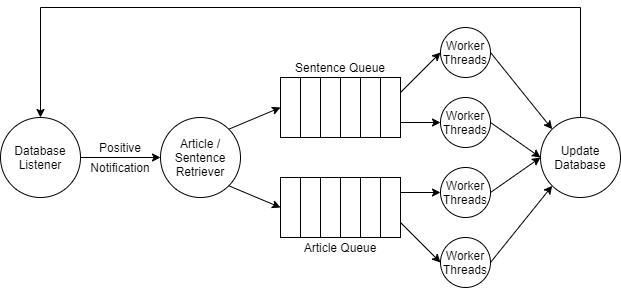
\includegraphics[width=0.5\linewidth]{images/upload/control.png}    
                \caption{Control component overview}
                \label{fig:control}
        \end{figure}
            
        Once the control component can communicate successfully with the backend components, it then setups a listener to be notified when articles are input into the system. When it receives a notification, it then splits any unfinished articles and sentences into two queues and uses multi-threading to process them. Once both queues are finished, the control component returns to listening for another notification. 
            
            \subsubsection{Listener}
            A core part of the control component is the database listener that awaits notification from the main database whenever an article or sentence is inserted into the system. This is done through a Postgres notification channel, which is set up on both the Article and Sentence tables. The control component listens to this channel, waiting for a notification to be broadcast. This prevents the component from needing to constantly poll the database for new articles and sentences.
           
            \subsubsection{Queue}
            Once a notification is received, the control component requests all unfinished articles and sentences from the database and creates a sentence and article queue. This queue is implemented using Python’s inbuilt Queue object and allows multiple worker threads to retrieve and complete tasks concurrently. 
            
            \subsubsection{Logic}
            Each worker thread uses a main sentence or article method that process an item according to its current status, see \ref{Main Database}. Each status is given a series of steps that utilize different backend components and then the database is updated. An overview of the control component’s logic can be seen in figure \ref{fig:control_logic} 
            
            \begin{figure}[!h]
                \centering
                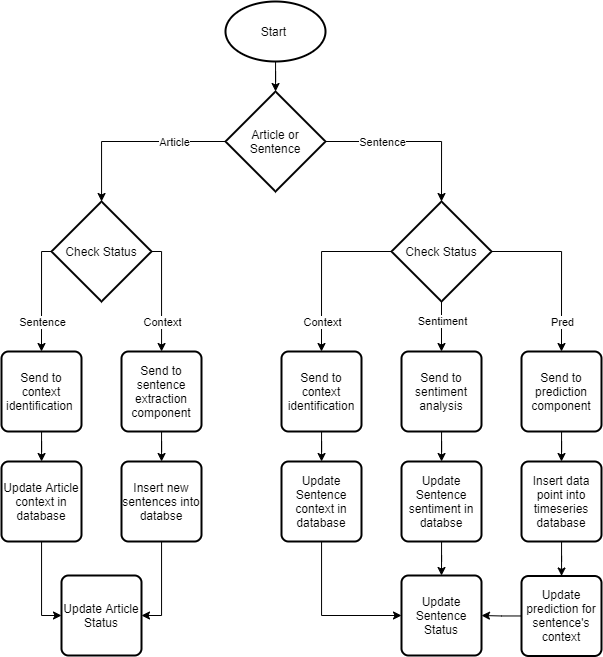
\includegraphics[width=0.4\linewidth]{images/upload/Logic Diagram.png}    
                \caption{Control component sentence and article process logic}
                \label{fig:control_logic}
            \end{figure}
            
    \section{Frontend Implementation}
    With the backend system operational, work could begin on the frontend system. An effective and user-friendly frontend system was crucial for the project and system to succeed and as such, much focus and time were spent improving and iterating on it. Django \citep{technology:Django} was the framework selected to build the frontend and its view and template building features allowed for data to be easily passed into and displayed to the website with little difficulty. 
    
        \subsection{Homepage}
        Before any stylization or features could be added to the homepage, the frontend first needed to be connected to the main database so that it could access the necessary data. Django comes connected to a Pymongo database, so it involved removing that connection and giving it the connection URL for the main database. Once the connection was successful, models were created for the Company, Sentences, Source and Tag tables in the main database. With the creation of these models, Django was able to generate its own API to the database. With the models complete, a simplistic version of the homepage was implemented to ensure that the database contents were being read correctly. This early implementation can be seen in Figure \ref{fig:Home_early}
            
        \begin{figure}[!h]
                \centering
                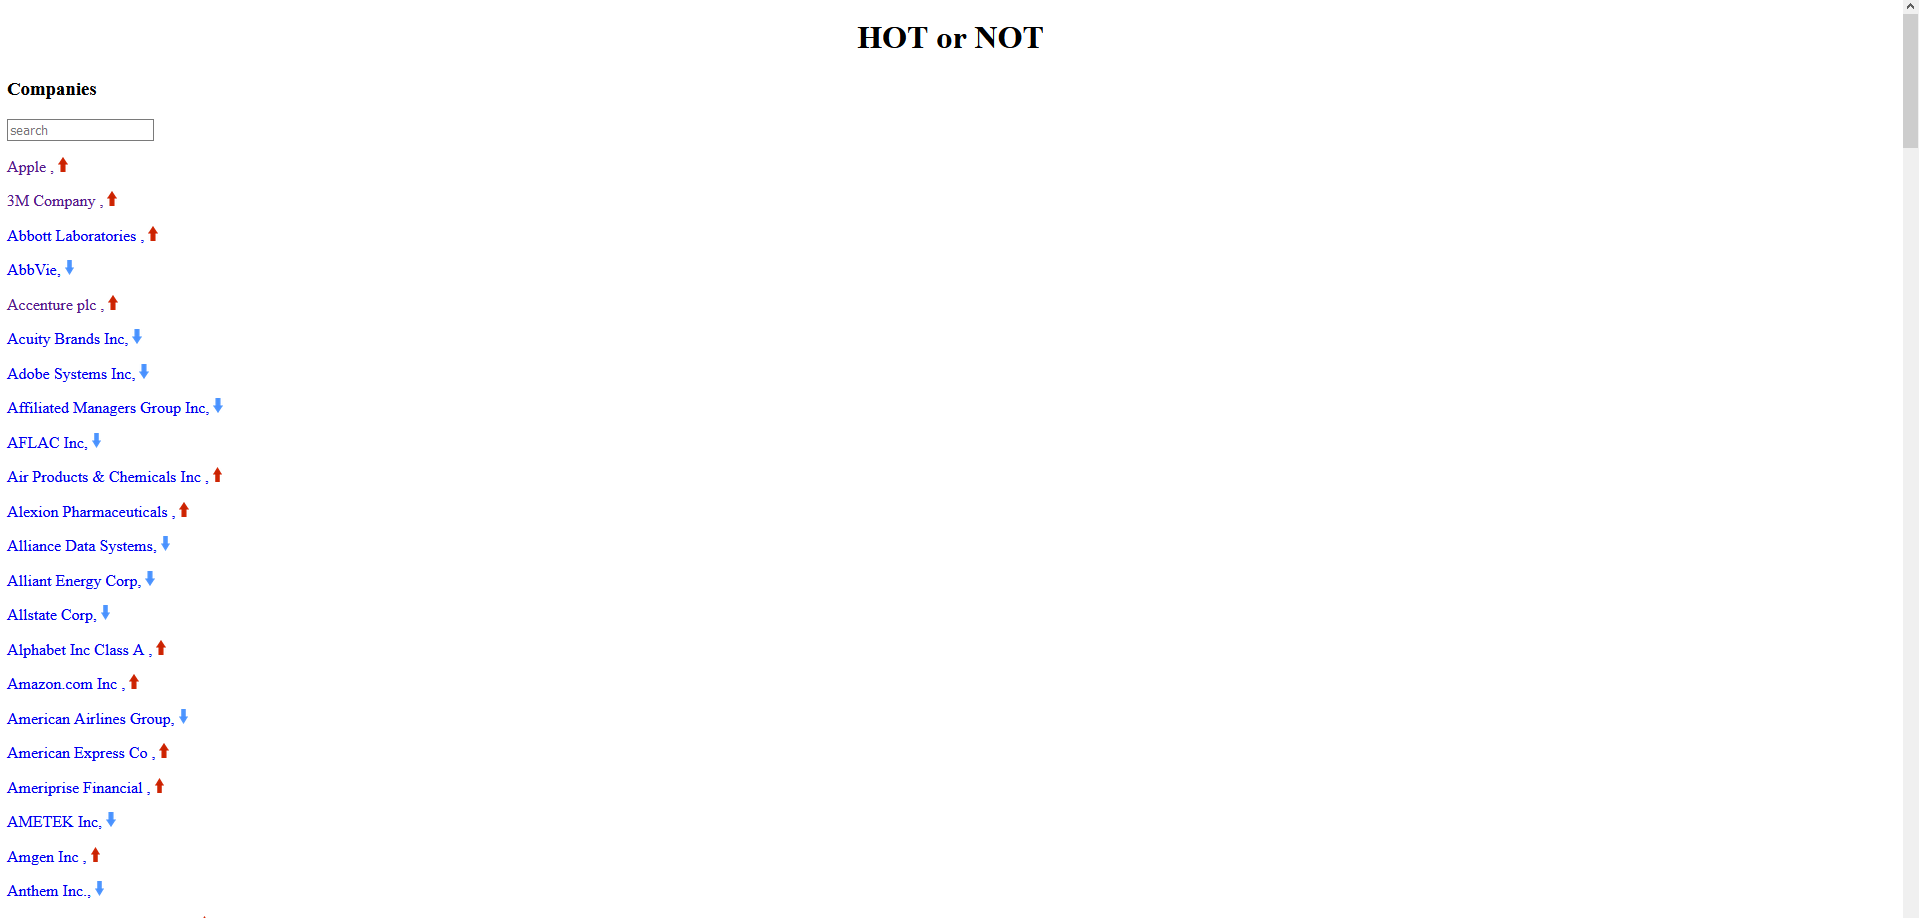
\includegraphics[width=0.5\linewidth]{images/upload/EarlyHome.png}    
                \caption{Early Implementation}
                \label{fig:Home_early}
        \end{figure}
            
        With Django fully connected to the database, the next stage implemented the designs discussed in chapter \ref{Design}
        
            \subsubsection{Company Card}
            As section \ref{Homepage} shows, each company on the homepage is given its card with styling according to its Hot or Not verdict. Initial work went into the arrangement and size of the boxes to achieve the three-column layout shown in the wireframes. With that achieved, work began on the styling and design of the company boxes. Each verdict was given its separate colour scheme and icon allowing the user to at a glance see which companies were hot and which were not. Next, the Hot or Not meter was implemented. This is based on the difference in the stock price mentioned in \ref{Verdict} and further allows the users to identify the difference between companies by seeing the degree to which they are hot or not. With the implementation of tags later in the project, the company boxes were extended to have small clickable tag buttons under the Hot or Not meter allowing the user to search and see other companies with the same tag. The company cards went through various design changes that saw the design improve through each iteration. The final implementation of the company cards can be seen in Figure \ref{fig:cards}. 
            
            \begin{figure}[!h]
            \begin{subfigure}[b]{0.5\textwidth}
                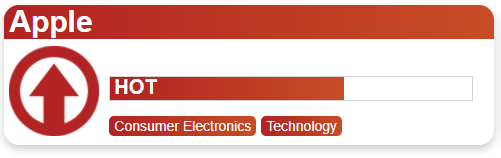
\includegraphics[width=\textwidth]{images/upload/card_hot.PNG}
                \caption{Company Card with hot status}
                \label{fig:card_hot}
            \end{subfigure}
            \hfill
            \begin{subfigure}[b]{0.5\textwidth}
                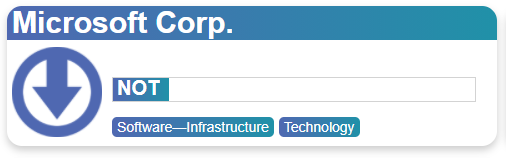
\includegraphics[width=\textwidth]{images/upload/card_not.png}
                \caption{Company Card with not status}
                \label{fig:card_not}
            \end{subfigure}
            \caption{Final implementation of the company cards}
            \label{fig:cards}
            \end{figure}
            
            \subsubsection{Search Bar}
            The search bar is perhaps the most important aspect of the homepage, as this is the main interface a potential user will use when attempting to find a company. Thanks to Djangos middleware API that is created from defined models, the frontend can easily perform queries on the main database to find any potential companies. With the implementation of tags, this search was also extended to search for companies that have similar tags to the ones that appear in the initial search. This allows not only for companies similar to the text typed by the user to appear, but also similar companies to appear.
            
            For the results of any search to be shown to the user without forcing a page to reload, AJAX was utilized to provide asynchronous updates to the homepage, changing the list of companies displayed from the database query. A sorting option was added under the search bar to allow the user to order the companies shown. The sorting options were easy to implement by simplifying the application of the sorting process for the found set of companies. The sort options given are Hot, Not, Hold, Alphabetical and stock code. Again, throughout the project's life-cycle, the search bar and the Homepage as a whole was updated and improved. The final version of the homepage can be seen in Figure\ref{fig:Home_final}
            
            \begin{figure}[!h]
                \centering
                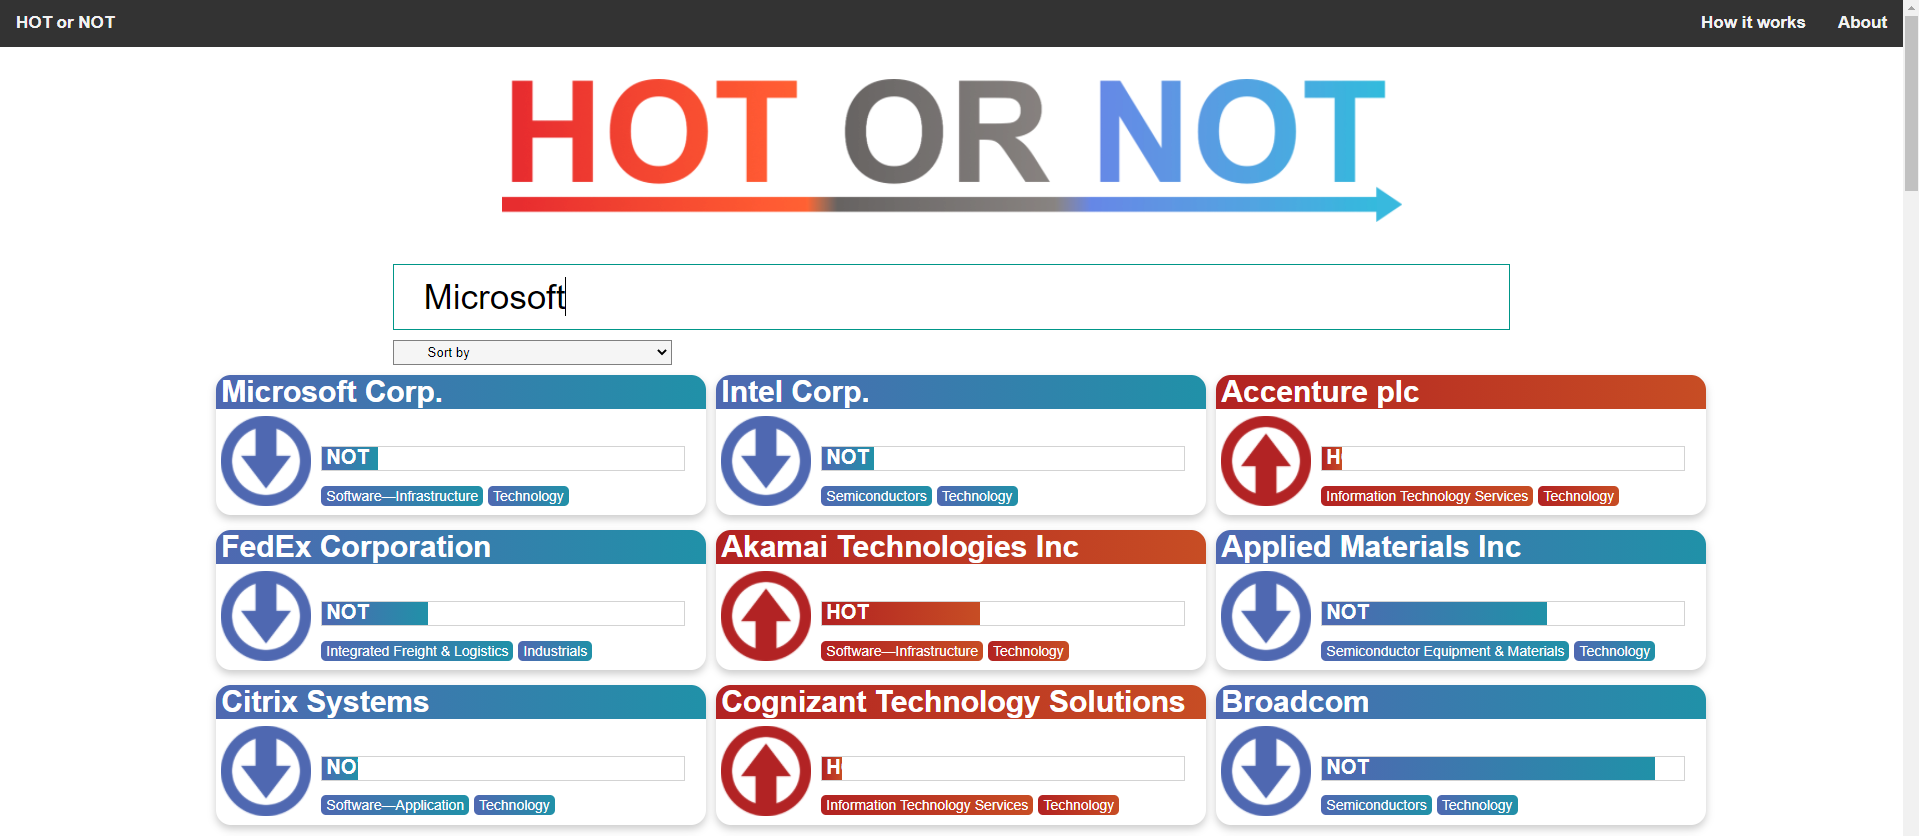
\includegraphics[width=0.9\linewidth]{images/upload/Homepage.PNG}
                \caption{Final version of the homepage}
                \label{fig:Home_final}
            \end{figure}
            
        
        \subsection{Company page}
        Once a user selects one of the company cards, they are taken to the company page. This page presents a variety of information about a given company; this information is separated into various tabs.
            
            \subsubsection{Our Predictions Tab}
            This tab stores the ready-made predictions made by the system and the verdict selection on each company is based on this. A graph of the historical stock price and predicted stock price is implemented using chartJS \citep{technology:Chartjs}, along with a chartJS extension that allows the user to drag and zoom into different areas of the chart.
            
            \subsubsection{Custom Prediction Tab}
            The custom predictions tab allows the user to create their predictions by selecting a start and end date. Firstly, to allow the user to enter the start and end date, a Django form was created that allows for safe data transfer from the webpage to the middle-ware. This form request, is processed using Ajax, sends a request to the stock prediction component containing the company stock code, along with the user defined start and end dates. The stock prediction component processes this request and returns the stock price prediction data. Thanks to Ajax, this data is then transferred to the webpage without needing to reload the page. Simply implementing chartJS and showing the custom predictions like how was done in the "Our Prediction Tab" was tried first, however there was a problem with transferring the python-generated data into the JavaScript chartJS. A small parser function was therefore created that allows the predictions to be transformed into data that works with chartJS, which is then displayed to the user. Later in the project, error handling was added to the stock prediction component and the custom prediction tab was modified to display error messages should something go wrong in the predictions. 
            
            \subsubsection{Article Snippets}
            With the majority of the core features implemented to the company page, work began on showing the article snippets for that company. A collapsible side section was added to the company page, allowing the user to view the twenty most recent sentences related to the company. To keep a consistent design throughout the webpage, the sentence boxes and section were designed to look similar to the company boxes shown on the homepage, having the same colour schemes and icons for Hot, Not and Hold sentences. Figure \ref{fig:snippets} shows the final implementation of the article snippets on the company page.
            
            \begin{figure}[!h]
                \centering
                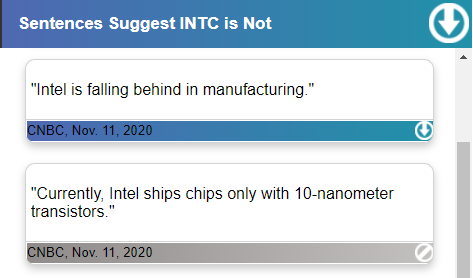
\includegraphics[width=0.5\linewidth]{images/upload/Snippets.PNG}
                \caption{Article sentence snippets}
                \label{fig:snippets}
            \end{figure}
            
            \subsubsection{Company Information Tab}
            The company information tab was originally home to basic information about the company and the different financial information on the company. However, although multiple designs and iterations to realize this tab were attempted, they did not achieve the standards of the rest of the websites and therefore it was felt that separating the tabs into "Company Profile" and "Financials" would allow for more specific designs that still remained consistent with the overall website design. The company profile and financial page all display information retrieved through the Yfiance \cite{technology:yfinance} library. The pages went through several iterations, with the final version, shown in Figure\ref{fig:info_page}, being in line with the overall style of the company page, while also displaying the information effectively. 
            
            \begin{figure}[!h]
            \begin{subfigure}[b]{0.5\textwidth}
                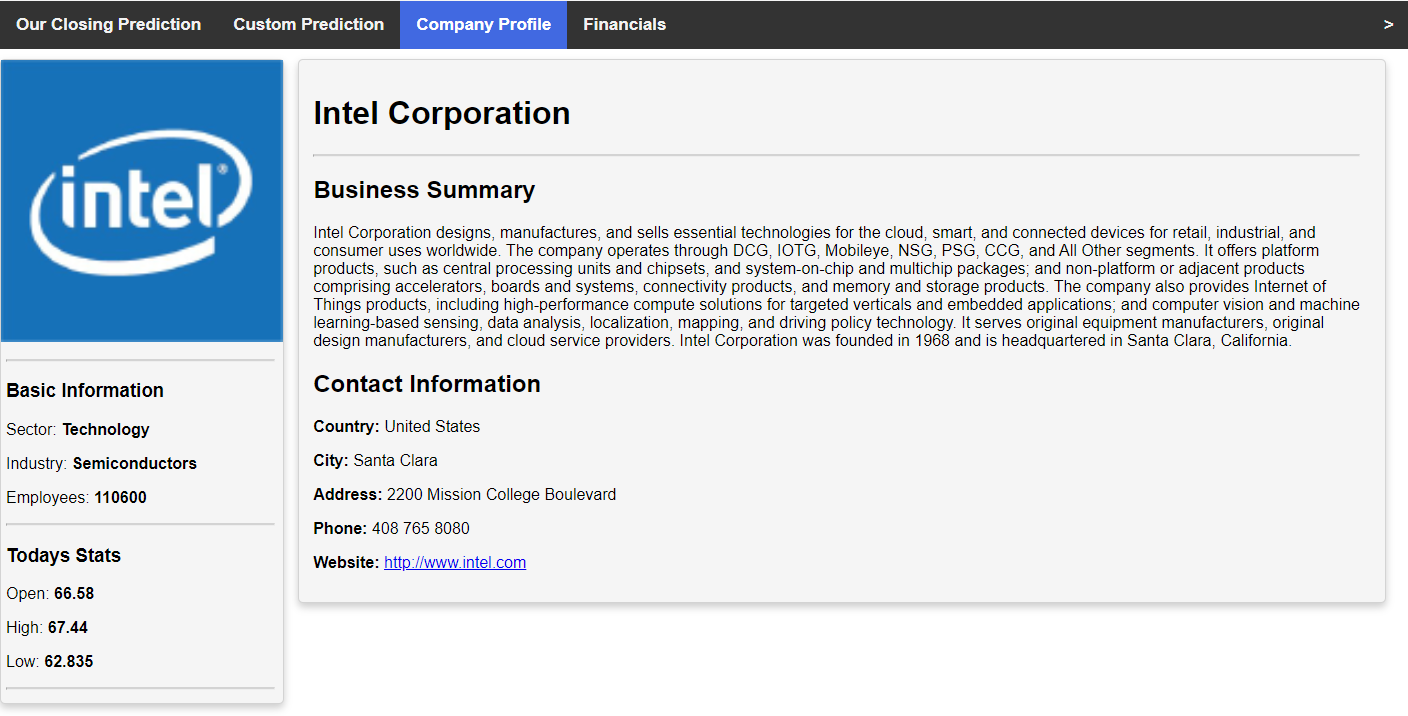
\includegraphics[width=\textwidth]{images/upload/CompanyInfo.PNG}
                \caption{Company Profile Tab}
                \label{fig:profile_tab}
            \end{subfigure}
            \hfill
            \begin{subfigure}[b]{0.5\textwidth}
                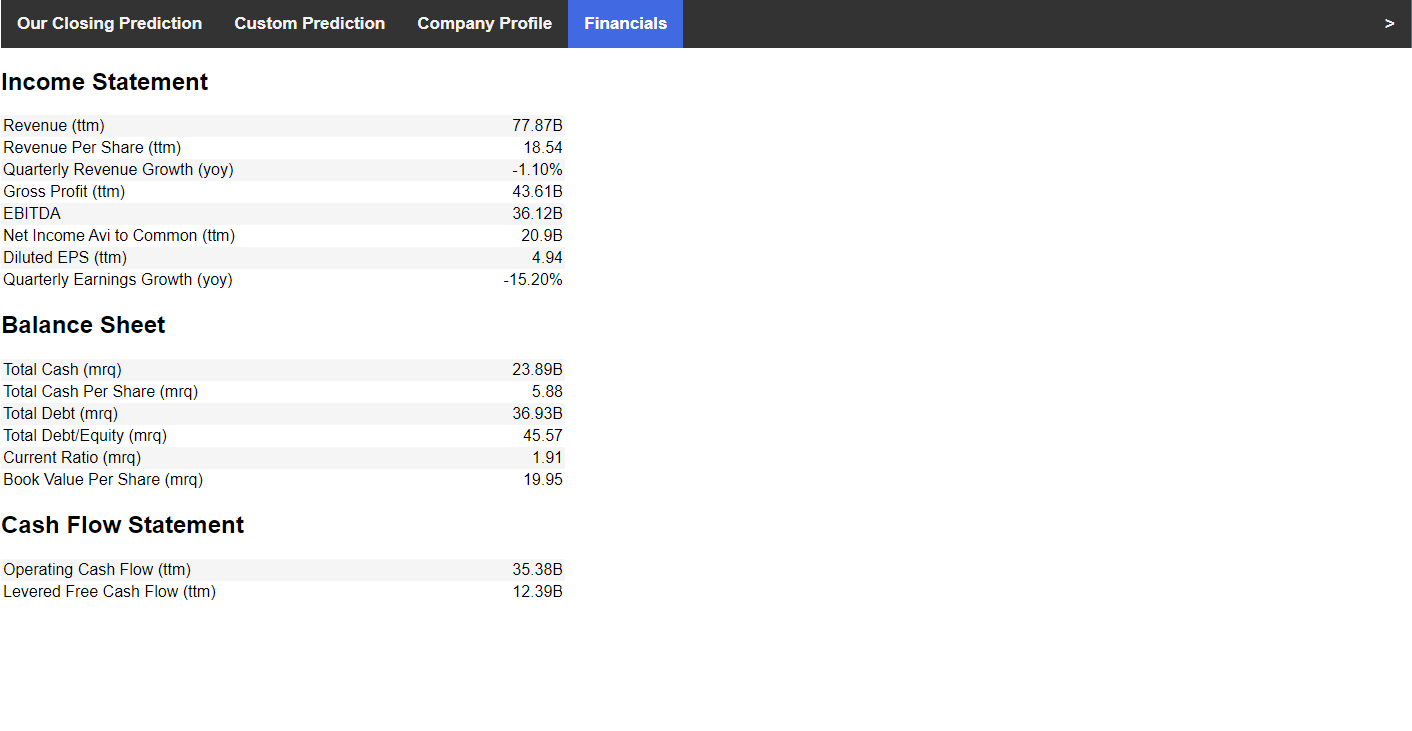
\includegraphics[width=\textwidth]{images/upload/Financial.PNG}
                \caption{Company Financial Tab}
                \label{fig:fin_tab}
            \end{subfigure}
            \caption{The company profile and financial tab of the company page}
            \label{fig:info_page}
            \end{figure}
            
            \subsubsection{AJAX} Then company page presents the user with a variety of information that both takes time to retrieve and needs constant updates, as is the case for the live stock price ticker. Therefore, it was important to shift some of the information displayed on the company page into asynchronous AJAX requests. When the company page first loads, two Ajxa requests to retrieve the financial and company information are made, which minimise some latency when loading the page. While the company page is loaded, it makes Ajax requests every five seconds to update the current stock price of the company. 
            
            \subsubsection{Overall}
            Navigating the separate tabs is done through the company page subheader that shows the company name, stock code and current stock price along with the various tabs that can be selected. The overall view of the page can be seen in Figure \ref{fig:Home_final}
            
            \begin{figure}[!h]
                \centering
                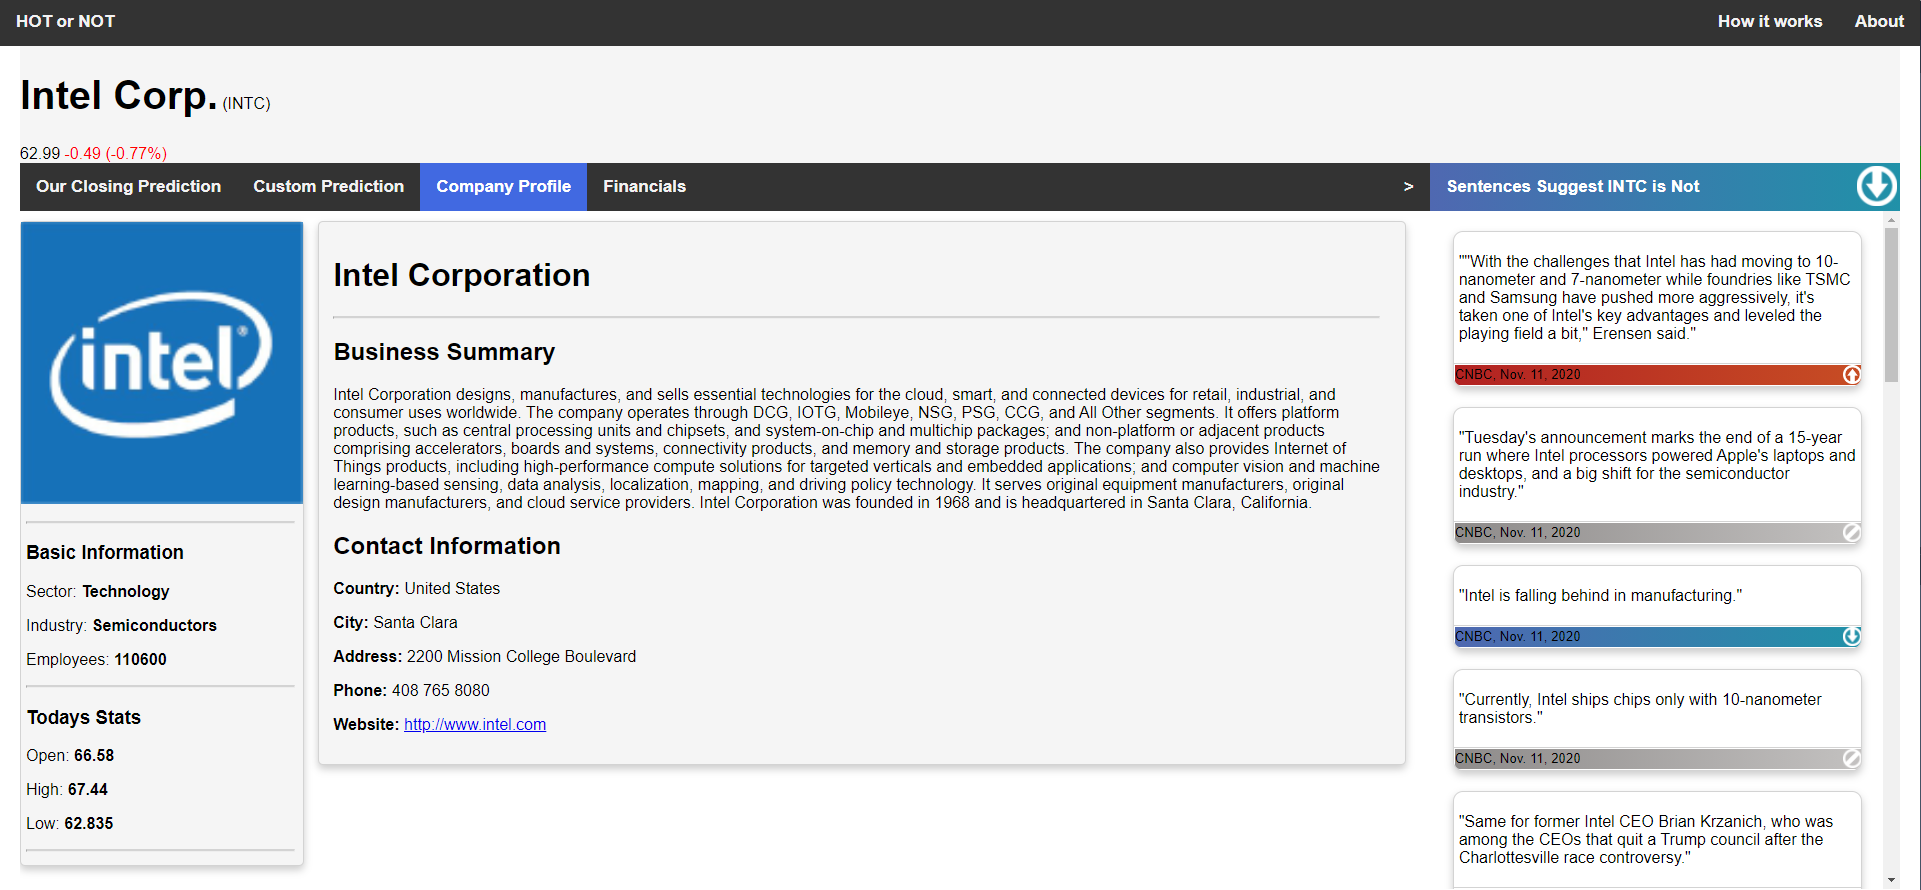
\includegraphics[width=0.9\linewidth]{images/upload/Comp_final.PNG}
                \caption{Final version of the company page}
                \label{fig:Home_final}
            \end{figure}
            
    
    \section{Containerization}
    %REDONE
    Once the system was fully working on a local level, it was important to have the project easily runnable on other machines and is a step towards to fully deploying the system. To achieve this, the various components of the system had to be implemented into containers and then connected. Docker \cite{merkel2014docker} was used to create the containers for the various components with the backend components, control component, backend API, main database, time-series database and frontend webapp all having separate containers. This meant creating requirement and Docker files across all the components, along with removing redundant data that would slow down build time. Containerizing the components went smoothly however, the main and time-series databases needed additional work. PostgreSQL and Timescale Docker base images had to be used as a starting point for the containers, with the exported SQL of the databases being imported during run time. Once the components worked individually, the next task was to tie them together using Docker Compose \citep{Jangla_2018}. Compose allows for containers to be combined into a single application increasing the ease of running the full system. A central Compose file was created detailing the Docker files for each component and their ID, run order and dependencies. Once the compose file was created, it was then a process of replacing the API call URL for each component with the new ID for the containers. 
            
    \section{Summary}
    This chapter details the steps, challenges and solutions in implementing the \textit{Hot or Not} system. The chapter highlights the software engineering practices used throughout the project and the benefit they had on the projects development. A description and justification of the technologies and steps taken to implement the backend, database and frontend systems along with how those separate components were integrated to create the overall working system. More information on the final deliverable can be found in Appendix \ref{Ap: Final Deliverable}.
    
    
    